%==============================================================================
% Sjabloon onderzoeksvoorstel bachproef
%==============================================================================
% Gebaseerd op document class `hogent-article'
% zie <https://github.com/HoGentTIN/latex-hogent-article>

% Voor een voorstel in het Engels: voeg de documentclass-optie [english] toe.
% Let op: kan enkel na toestemming van de bachelorproefcoördinator!
\documentclass{hogent-article}

% Invoegen bibliografiebestand
\addbibresource{voorstel.bib}

% Informatie over de opleiding, het vak en soort opdracht
\studyprogramme{Professionele bachelor toegepaste informatica}
\course{Bachelorproef}
\assignmenttype{Onderzoeksvoorstel}
% Voor een voorstel in het Engels, haal de volgende 3 regels uit commentaar
% \studyprogramme{Bachelor of applied information technology}
% \course{Bachelor thesis}
% \assignmenttype{Research proposal}

\academicyear{2022-2023} % TODO: pas het academiejaar aan

% TODO: Werktitel
\title{Tracking van koeien en identificatie van hun gedrag}

% TODO: Studentnaam en emailadres invullen
\author{Tomma Vlaemynck}
\email{tomma.vlaemynck@student.hogent.be}

% TODO: Medestudent
% Gaat het om een bachelorproef in samenwerking met een student in een andere
% opleiding? Geef dan de naam en emailadres hier
% \author{Yasmine Alaoui (naam opleiding)}
% \email{yasmine.alaoui@student.hogent.be}

% TODO: Geef de co-promotor op
\supervisor[Co-promotor]{J. Haumont (Ilvo, \href{mailto:jeremie.haumont@ilvo.vlaanderen.be}{jeremie.haumont@ilvo.vlaanderen.be})}

% Binnen welke specialisatierichting uit 3TI situeert dit onderzoek zich?
% Kies uit deze lijst:
%
% - Mobile \& Enterprise development
% - AI \& Data Engineering
% - Functional \& Business Analysis
% - System \& Network Administrator
% - Mainframe Expert
% - Als het onderzoek niet past binnen een van deze domeinen specifieer je deze
%   zelf
%
\specialisation{AI \& Data Engineering}
\keywords{Localisatie , Identificatie, $\lambda$-calculus}

\begin{document}

\begin{abstract}
  Hier schrijf je de samenvatting van je voorstel, als een doorlopende tekst van één paragraaf. Let op: dit is geen inleiding, maar een samenvattende tekst van heel je voorstel met inleiding (voorstelling, kaderen thema), probleemstelling en centrale onderzoeksvraag, onderzoeksdoelstelling (wat zie je als het concrete resultaat van je bachelorproef?), voorgestelde methodologie, verwachte resultaten en meerwaarde van dit onderzoek (wat heeft de doelgroep aan het resultaat?).
\end{abstract}

\tableofcontents

% De hoofdtekst van het voorstel zit in een apart bestand, zodat het makkelijk
% kan opgenomen worden in de bijlagen van de bachelorproef zelf.
%---------- Inleiding ---------------------------------------------------------

\section{Introductie}%
\label{sec:introductie}

In dit onderzoeksvoorstel, uitgevoerd bij ILVO, worden geavanceerde mogelijkheden van technologieën verkend voor het volgen en begrijpen van koeiengedrag in de moderne veehouderij. 
Het correct volgen en identificeren van gedrag van koeien is van cruciaal belang, niet alleen voor het welzijn van de dieren, maar ook voor de operationele efficiëntie van boerderijen. 
Deze studie richt zich op het analyseren van verschillende technologische methoden, waaronder objectdetectie en diepteschatting, om de locatie van koeien te bepalen en gedragingen zoals grazen, wandelen en rusten te identificeren. We onderzoeken de praktische uitdagingen en kansen die deze technologieën bieden in een agrarische omgeving. 
Het doel is om een diepgaand inzicht te krijgen in hoe deze technologische vooruitgang kan leiden tot verbeteringen in veehouderijpraktijken, met een specifieke focus op de impact op dierenwelzijn en boerderijbeheer. 
Dit onderzoek zal niet alleen bijdragen aan de wetenschappelijke kennis over diergedrag en technologische toepassingen in de landbouw, maar ook praktische richtlijnen bieden voor implementatie in de sector, wat de weg vrijmaakt voor innovatieve oplossingen in de toekomst van de landbouw.
%---------- Stand van zaken ---------------------------------------------------

\section{Literatuurstudie}%
\label{sec:state-of-the-art}
De technologische vooruitgang in de veehouderij heeft een nieuwe dimensie toegevoegd aan het volgen en analyseren van vee. 
De integratie van GPS- en RFID-technologieën, zoals onderzocht door \cite{Nääs2013} en \cite{Akhigbe2021}, heeft de basis gelegd voor efficiëntere trackingmethoden. 
Deze technologieën spelen een cruciale rol in het bieden van inzicht in de bewegingen en het gedrag van vee, wat essentieel is voor het beheer van hun gezondheid en welzijn.
Ontwikkelingen in computervisie en machine learning hebben nieuwe mogelijkheden geopend voor real-time monitoring en gedragsanalyse, zoals benadrukt door \cite{Kleanthous2018}. 
Geavanceerde technieken zoals objectdetectie en keypoints-analyse bieden gedetailleerde inzichten in het gedrag van vee, wat van groot belang is voor hun welzijnsbeoordeling. 
De toepassing van 3D-beeldvormings-technologieën, onderzocht \\door \cite{LeCozler2019}, heeft de precisie in het volgen en analyseren van vee verder verhoogd.
Deze methoden stellen ons in staat om gedetailleerde informatie te verzamelen, wat cruciaal is voor het beoordelen van de fysieke gezondheid van het vee.
Echter brengen deze ontwikkelingen ook uitdagingen met zich mee, zoals het identificeren van gedrag in verschillende omgevingscondities en het handhaven van nauwkeurigheid in complexe landbouwomgevingen \autocite{Narayan2023}\autocite{Busse2015}. 
Het is belangrijk om een evenwicht te vinden tussen het gebruik van geavanceerde technologieën en het waarborgen van dierenwelzijn en duurzaamheid.
Deze studies onderstrepen de vooruitgang en de voortdurende behoefte aan onderzoek en ontwikkeling in de implementatie en effectiviteit van technologieën. 
De integratie van deze technologieën belooft een efficiënte en diergerichte toekomst voor de veehouderij.
%---------- Methodologie ------------------------------------------------------
\section{Methodologie}%
\label{sec:methodologie}
Fasen van het onderzoek:
\begin{itemize}
  \item Fase 1: Literatuurstudie (2 week)
  \item Fase 2: Datacollectie (2 weken)
  \item Fase 3: Technologieën en Technieken (3 weken)
  \item Fase 4: Data-analyse en -verwerking (3 weken)
  \item Fase 5: Integratie en Evaluatie (2 weken)
  \item Fase 6: Conclusie (2 weken)
\end{itemize}
\subsection{Literatuurstudie}
Deze fase richt zich op het verkrijgen van een kennis van de huidige stand van zaken in de technologieën voor vee tracking. 
De focus ligt op het analyseren van studies over machine learning en computervisie. 
Hierbij is het doel het identificeren van de meest effectieve methoden en technieken voor gedragsanalyse van vee.
\end{itemize}
\subsection{Datacollectie}
In deze fase richt het onderzoek zich op de collectie van real-time gedragsdata van koeien met behulp van camera's. 
Het doel is om methoden voor data-extractie en -beheer te verkennen en te analyseren. 
De focus ligt op het opzetten van geautomatiseerde data pipelines, terwijl tegelijkertijd de bestaande technologieën en datasets van ILVO worden onderzocht. 
Dit onderzoek zal bepalen of en hoe ILVO's huidige middelen kunnen bijdragen aan de verrijking en uitbreiding van de verzamelde data. 
Elke stap in dit proces zal worden onderbouwd met zorgvuldig onderzoek, om te verzekeren dat de aanpak zowel wetenschappelijk gefundeerd als praktisch haalbaar is.
\end{itemize}
\subsection{Technologieën en Technieken}
De focus van dit onderdeel is de selectie en integratie van de meest geschikte technologieën voor de gedetailleerde analyse van koeiengedrag.
Dit proces omvat de aanpassing en toepassing van diverse bestaande computervisietechnieken.
  \begin{itemize}
    \item Objectdetectie: We zullen geavanceerde object-
    detectie-algoritmen zoals YOLO, SSD en Faster R-CNN inzetten. Deze technieken zijn cruciaal voor het nauwkeurig identificeren en lokaliseren van koeien binnen videobeelden, wat de basis vormt voor verdere gedragsanalyse.
    \item Keypoints-analyse: Voor de gedetailleerde analyse van bewegingen en houdingen van koeien, zullen keypoints-analyse technieken zoals OpenPose en AlphaPose worden gebruikt. Deze technieken stellen ons in staat om specifieke punten op het lichaam van de koe te identificeren en te volgen, wat essentieel is voor het begrijpen van hun gedrag.
    \item Bewegingsanalyse: Door de toepassing van optische stroming en tracking-algoritmen kunnen we de bewegingen van koeien over tijd volgen. Dit helpt ons om patronen in hun beweging te herkennen en te analyseren.
    \item Gedragsclassificatie: Machine learning en deep learning technieken zullen worden gebruikt voor de classificatie van specifieke gedragingen. Dit stelt ons in staat om verschillende gedragspatronen te identificeren en te categoriseren, van eenvoudige acties tot complexe sociale interacties.
    \item Anomaliedetectie: Tot slot zullen we anomalie
    detectie-technieken inzetten om afwijkingen van normaal gedrag te identificeren, wat kan wijzen op gezondheidsproblemen of stress bij de koeien.
  \end{itemize}
Deze geïntegreerde aanpak combineert meerdere computervisietechnieken om een uitgebreid en nauwkeurig beeld te krijgen van het gedrag van koeien. De keuze voor specifieke technologieën en de integratiestrategie zal worden onderbouwd door uitgebreid onderzoek en analyse, om de effectiviteit en nauwkeurigheid van de gedragsanalyse te maximaliseren.
\end{itemize}
\subsection{Data-analyse en -verwerking}
In de data-analyse en -verwerkingsfase van de bachelorproef wordt gebruik gemaakt van geavanceerde machine learning algoritmen om koeiengedrag te analyseren en te classificeren.
De focus ligt op de volgende aspecten:
  \begin{itemize}
    \item Selectie van Algoritmen: We zullen specifieke machine learning algoritmen kiezen die het best passen bij onze data en analysebehoeften. Dit kan variëren van Convolutional Neural Networks (CNNs), die effectief zijn voor beeldclassificatie en herkenning, tot Recurrent Neural Networks (RNNs) die geschikt zijn voor het analyseren van tijdsafhankelijke data. Afhankelijk van de complexiteit van de gedragspatronen, kunnen ook eenvoudigere algoritmen zoals Decision Trees of Support Vector Machines (SVMs) worden overwogen.
    \item Training en Optimalisatie: Zodra de algoritmen zijn geselecteerd, worden deze getraind met de verzamelde data. Dit proces omvat het afstellen van parameters en het toepassen van technieken zoals cross-validation om de effectiviteit van de modellen te maximaliseren.
    \item Validatie: Na het trainen van de modellen is het essentieel om hun prestaties te testen en valideren met nieuwe, ongeziene data. Dit helpt ons om de nauwkeurigheid en betrouwbaarheid van de modellen te beoordelen.
  \end{itemize}
Deze aanpak zorgt ervoor dat we diepgaande en betrouwbare inzichten verkrijgen in koeiengedrag, ondersteund door robuuste data-analyse en \\-verwerkingstechnieken.
\end{itemize}
\subsection{Integratie en Evaluatie}
Implementatie en toetsing van de ontwikkelde technieken en modellen in een realistische landbouwomgeving. 
Beoordeling van de effectiviteit, nauwkeurigheid en bruikbaarheid van de technologieën. 
\subsection{Conclusie}
Reflectie op de resultaten van het onderzoek, met een nadruk op de impact van de geïntegreerde technologieën en methoden op de veehouderijpraktijk. 
Aanbevelingen voor toekomstig onderzoek en mogelijke verbeteringen.
\subsection{Gantt-chart}
\newline
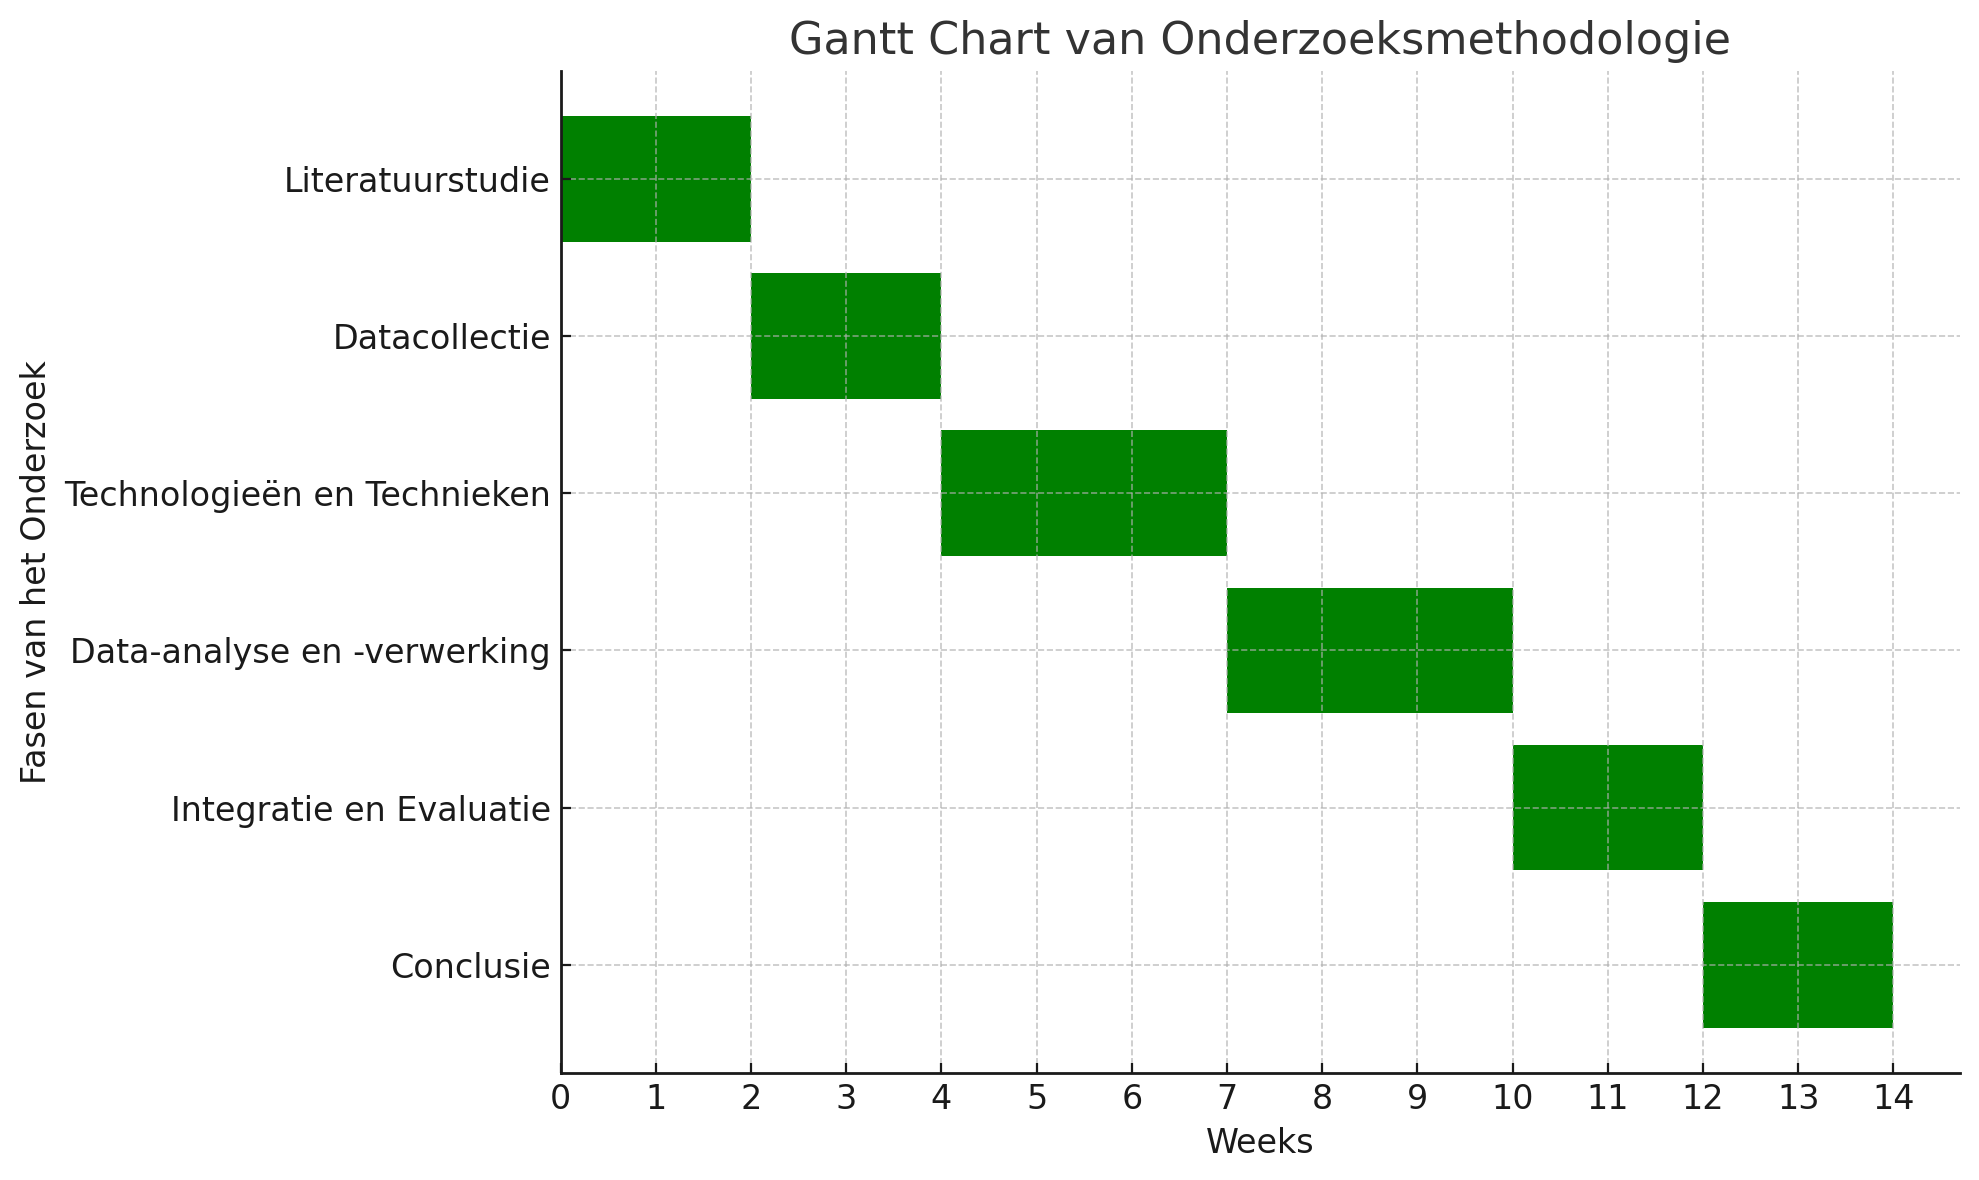
\includegraphics[width=\linewidth]{gantt_chart.png}
\newline
%---------- Verwachte resultaten ----------------------------------------------
\section{Verwacht resultaat, conclusie}%
\label{sec:verwachte_resultaten}
In dit onderzoek verwachten we de volgende resultaten te verkrijgen:
\begin{itemize}
  \item Verbeterde nauwkeurigheid in het monitoren van koeiengedrag door geavanceerde technologieën, zoals objectdetectie en \newline keypoints-analyse, toe te passen.
  \item Efficiëntere methoden voor gedragsanalyse van koeien in verschillende omgevingsomstandigheden.
  \item Geavanceerde Analytische Inzichten: In plaats van een geïntegreerd systeem voor locatie- en gedragsvolging, zal de focus liggen op het ontwikkelen van geavanceerde analytische inzichten die de basis leggen voor toekomstige integratie in dergelijke systemen. Het doel is om diepgaande kennis te verwerven over koeiengedrag, wat cruciaal is voor het ontwerpen van effectieve monitoringssystemen.
\end{itemize}
Deze resultaten zullen een meerwaarde bieden voor de veehouderij door bij te dragen aan het welzijn van dieren en de operationele efficiëntie te verbeteren. Het gebruik van geavanceerde technologieën voor gedragsmonitoring kan leiden tot betere besluitvorming en zorg voor het vee, en uiteindelijk tot positieve economische en ethische gevolgen voor de landbouwsector.

Het is belangrijk op te merken dat de uiteindelijke resultaten kunnen variëren op basis van de uitkomsten van de data-analyse en evaluatie van de gebruikte technologieën. 
Dit onderzoek zal een grondige analyse bieden om eventuele afwijkingen te verklaren en aanbevelingen te doen voor verdere verbeteringen.


\printbibliography[heading=bibintoc]

\end{document}